\documentclass{csse4400}

% \teachermodetrue

\usepackage{float}

\usepackage{languages}

\title{Empty Practical}
\author{Evan Hughes \& Brae Webb}

\date{\week{0}}
\begin{document}

\maketitle

\section{This Week}
This week our goal is to:
\begin{itemize}
  \item Deploy our TaskOverflow Application with a Load Balancer.
  \item Deploy a Autoscaling architecture on EC2.
  \item Deploy a Autoscaling architecture on ECS. 
\end{itemize}

\section{Load Balancers}

\todo{General overview of the topic}

\subsection{Routing Algorithms}

\begin{description}
  \item[Round Robin] This method allocates to the next available server no matter who the last request was sent to. Even though it may feel too simple it in practice works very effectively.
  \item[Least Connections] This method the load balancer keeps track of how many connections has been allocated to each node. It then sends the next request to the node with the least connections.
  \item[Weighted Least Connections] Similar to Least Connections but has a weight associated with each node. This allows us to preference certain nodes over others. An example of where this could be used is if we have a new node that we have added which is less powerful than the other nodes and we want to give it less load.
  \item[Consistent Hashing] In some cases we may want a user to continously be routed to a specific node. This is useful for multiple transactions that need to be done in a consistent order or if the data is stored/cached on the node. This can be done by hashing the information in the request payload or headers and then rout the request to the node that looks after that hash group.
  \item[Others...] Many more algorithms exist wether generic or bespoke for an application. 
\end{description}

\subsection{Health Checks}

An important aspect of load balancing is to ensure that the nodes that we route to are actually able to service the request. A strong health check can save or break your service depending on how you plan it, consider the two following examples which have happened within ITS:\\

\textbf{Example 1:} At the start of my career (Evan Hughes) I setup a multi-node Directory Server at UQ under the hostname of ldap.uq.edu.au, which is effectively a NoSQL database implementing the LDAP protocol, widely used for authentication services. This service is one that underpins UQ Authenticate which provides Single Sign-On for UQ. The service is setup with a load balancer that checks that port 389 is open and available to the load balancer.  This works for some time but an outage accurs in the data-center such that the disk of the OS running the service has dissapeared but the service is still running in memory. Even though upstream systems of the LDAP service have switched to the healthy data center they still talk to the dead nodes of LDAP due to the health check being too weak.\\

\todo{C4 Diagram of the architecture}

\textbf{Example 2:} During the rollout of a new prompt for UQ Authenticate which required users to go to My.UQ to provide verified contact details the Blackboard (learn.uq.edu.au) service went completly offline. The health check for Blackboard at the time actually did a full authentication as a test user to ensure everything was functioning as expected. Once this user was enrolled into the new campaign the health checks started going offline and within a matter of minutes the entire pool of nodes were shutdown. This health check was too wide and was not specific enough to the service that it was checking.\\

\todo{C4 diagram of the architecture}

A lot of services will provide a health check endpoint or a metrics endpoint which can help the engineer setup a proper level of health check. We want a health check that is specific enough for the service that it is checking but not so specific that it is too brittle. For the TaskOverflow application that we have been building so far, a reasonable health check would be that the health endpoint ensures the database is available and that the application is able to connect to it.

\section{Load Balancers in AWS}

Not all load balancers are alike, some usecases can require inspection into the packets being transmitted to make the correct choice of where it should go. In AWS we have two types of load balancers that we are going to cover.

\begin{description}
  \item[Application Load Balancer] This is a layer 7 load balancer that can route based on the content of the request. This is useful for services that are using HTTP, HTTPS or any other supported protocol.
  \item[Network Load Balancer] This is a layer 4 load balancer that can route based on the source and destination IP addresses and ports. This is useful for services that are using TCP or UDP.
\end{description}

The design of the load balancer is described in the diagram below with three destinct components. 

\begin{description}
  \item[Listeners] Listeners are the doors on the load balancer that allow traffic to enter. Each listener has a port and a protocol associated with it. For example we can have a listener with a port of 80 and a protocol of HTTP.
  \item[Target Groups] Target groups are the groups of nodes that the load balancer can route to. Each target group also has a protocol and a port associated with it. This allows us to switch ports on the way through the load balancer if the targets are using a different port to what we wish to expose.
  \item[Load Balancer] The load balancer is the actual load balancer that routes the traffic to the target groups based on rules that we setup. The load balancer has a DNS name that we can use to route traffic to it. The load balancer also has a security group that we can use to control what traffic can enter the load balancer. 
\end{description}

\begin{figure}[H]
  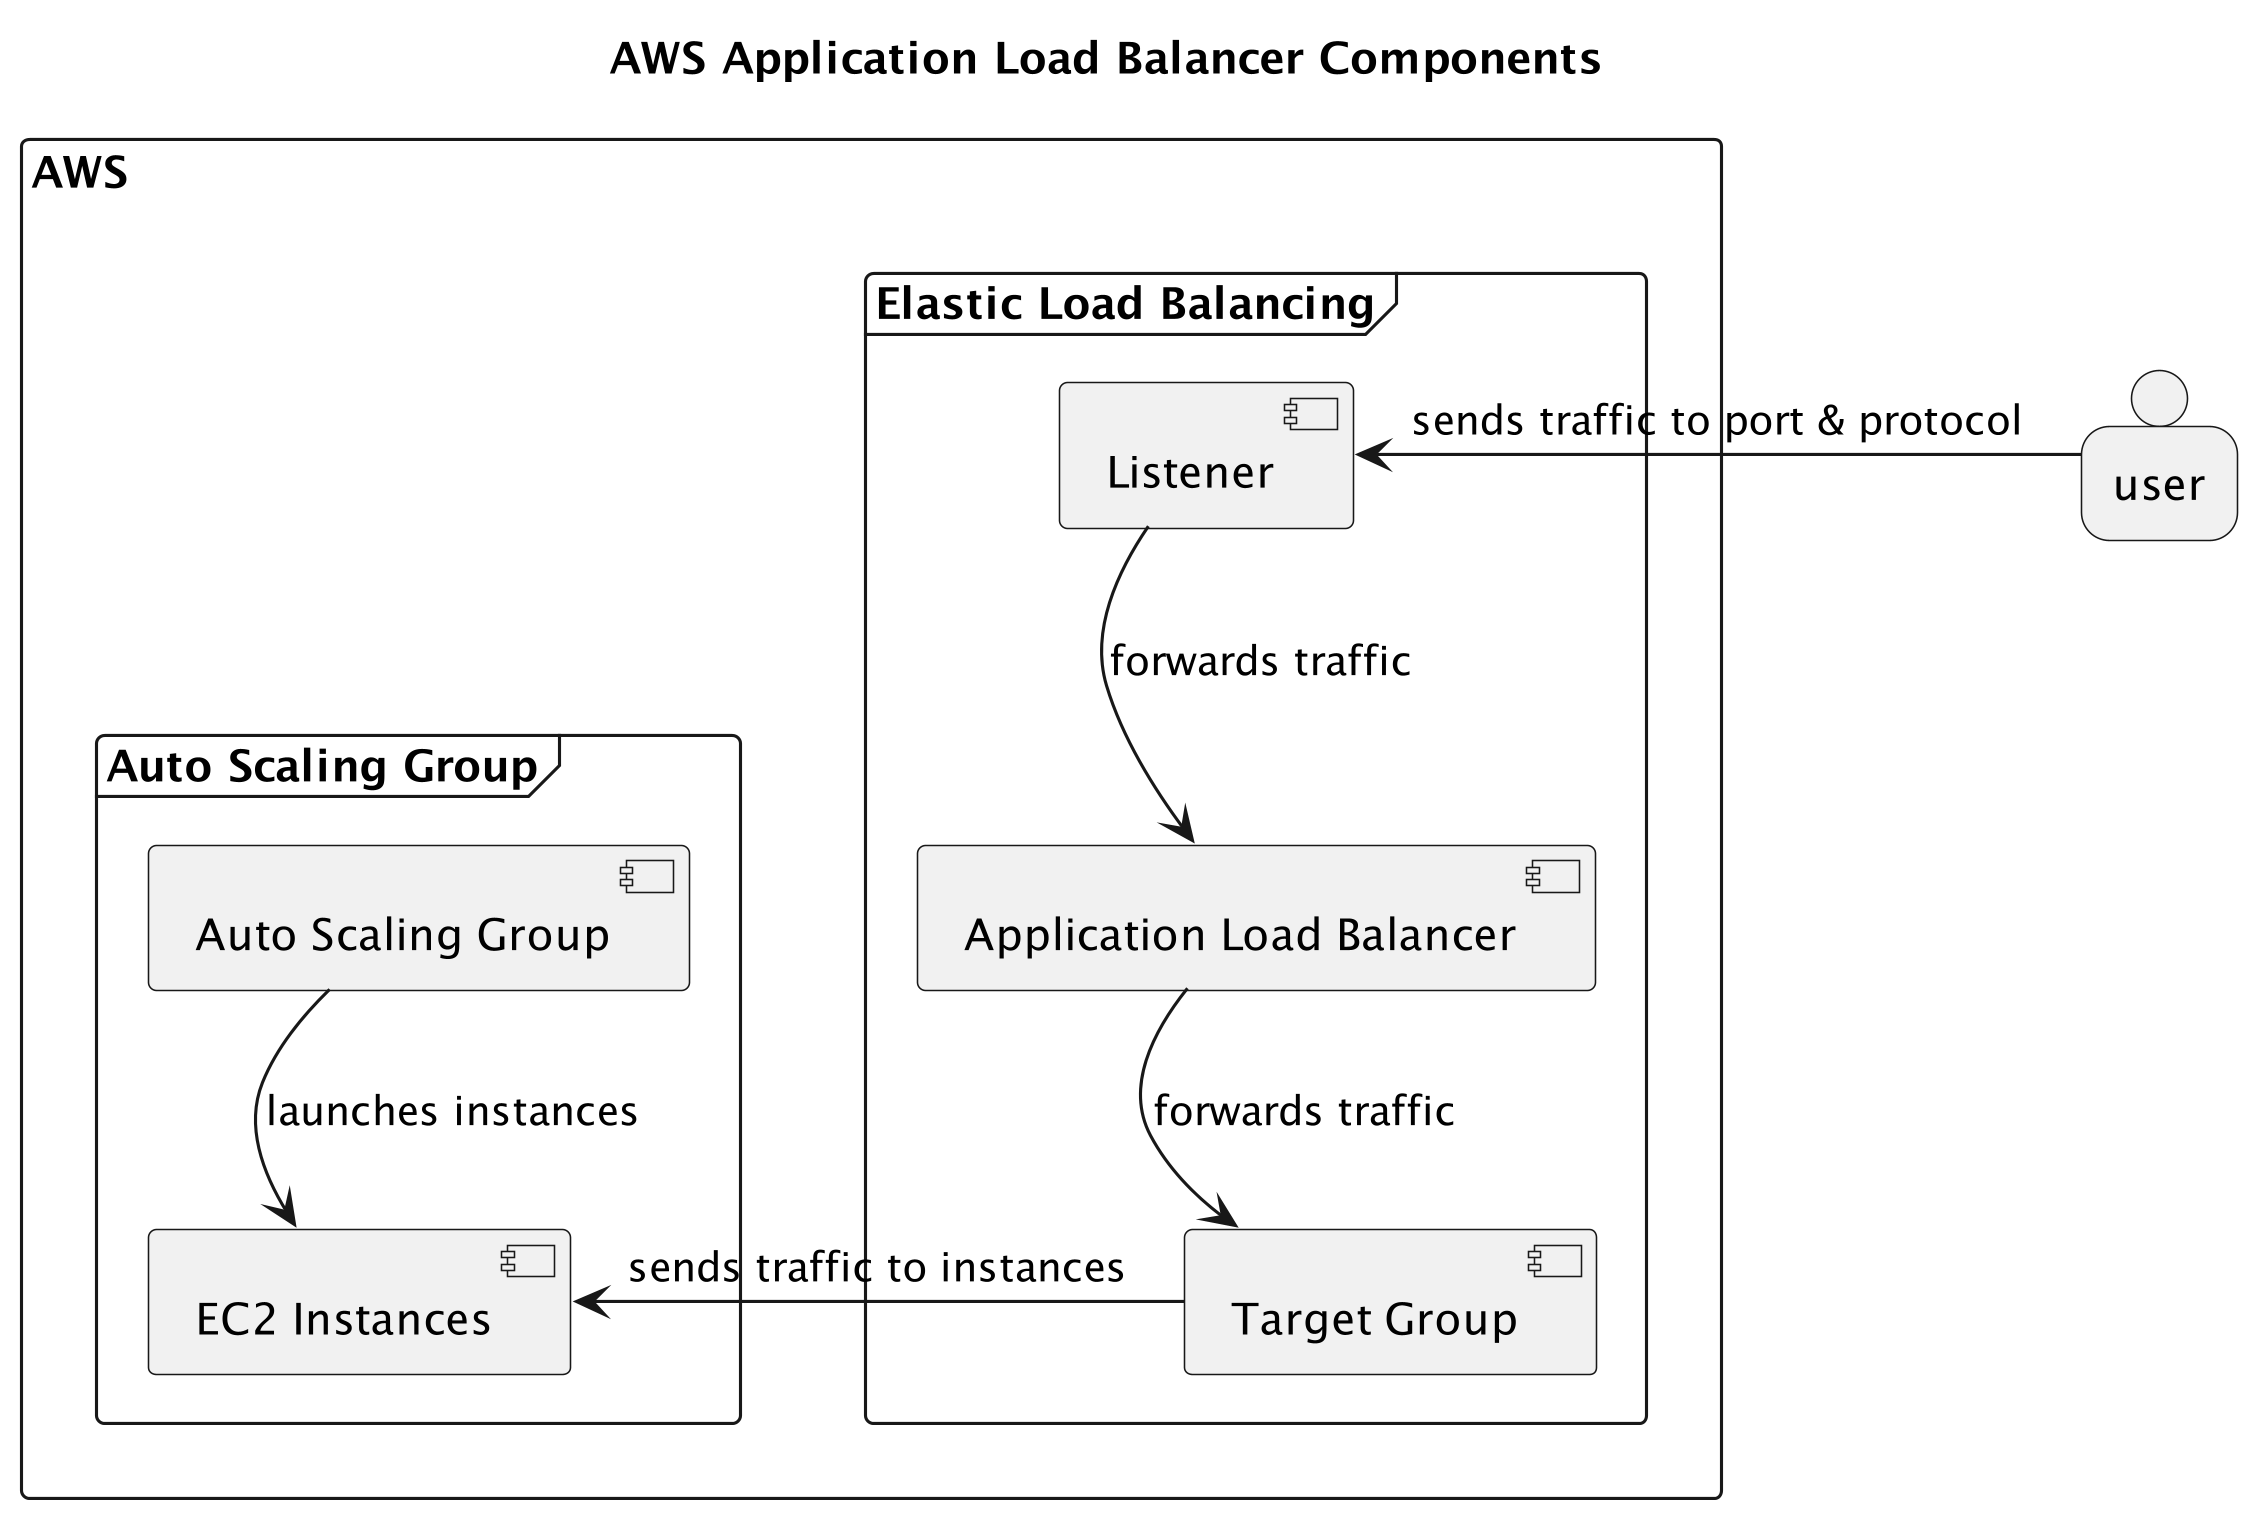
\includegraphics[width=\textwidth]{diagrams/loadbalancers}
\end{figure}

\section{Autoscaling in AWS}

As load balancers are able to distribute load we need to be able to have nodes that can service the load. Instead of having to create the maxiumum amount of services we predict will need we can utilise autoscaling to minimise resources when load is low and scale up when load is high. For compute resources in AWS this is mostly down around triggers from CloudWatch and scaling policies. Some of the premade triggers are based around the CPU usage of the node, the memory usage of the node and the network usage of the node. We can also create custom triggers based on the metrics that we are collecting from our application.

\section{Load Balancing TaskOverflow}

\subsection{[Path A] EC2}

\begin{figure}[H]
  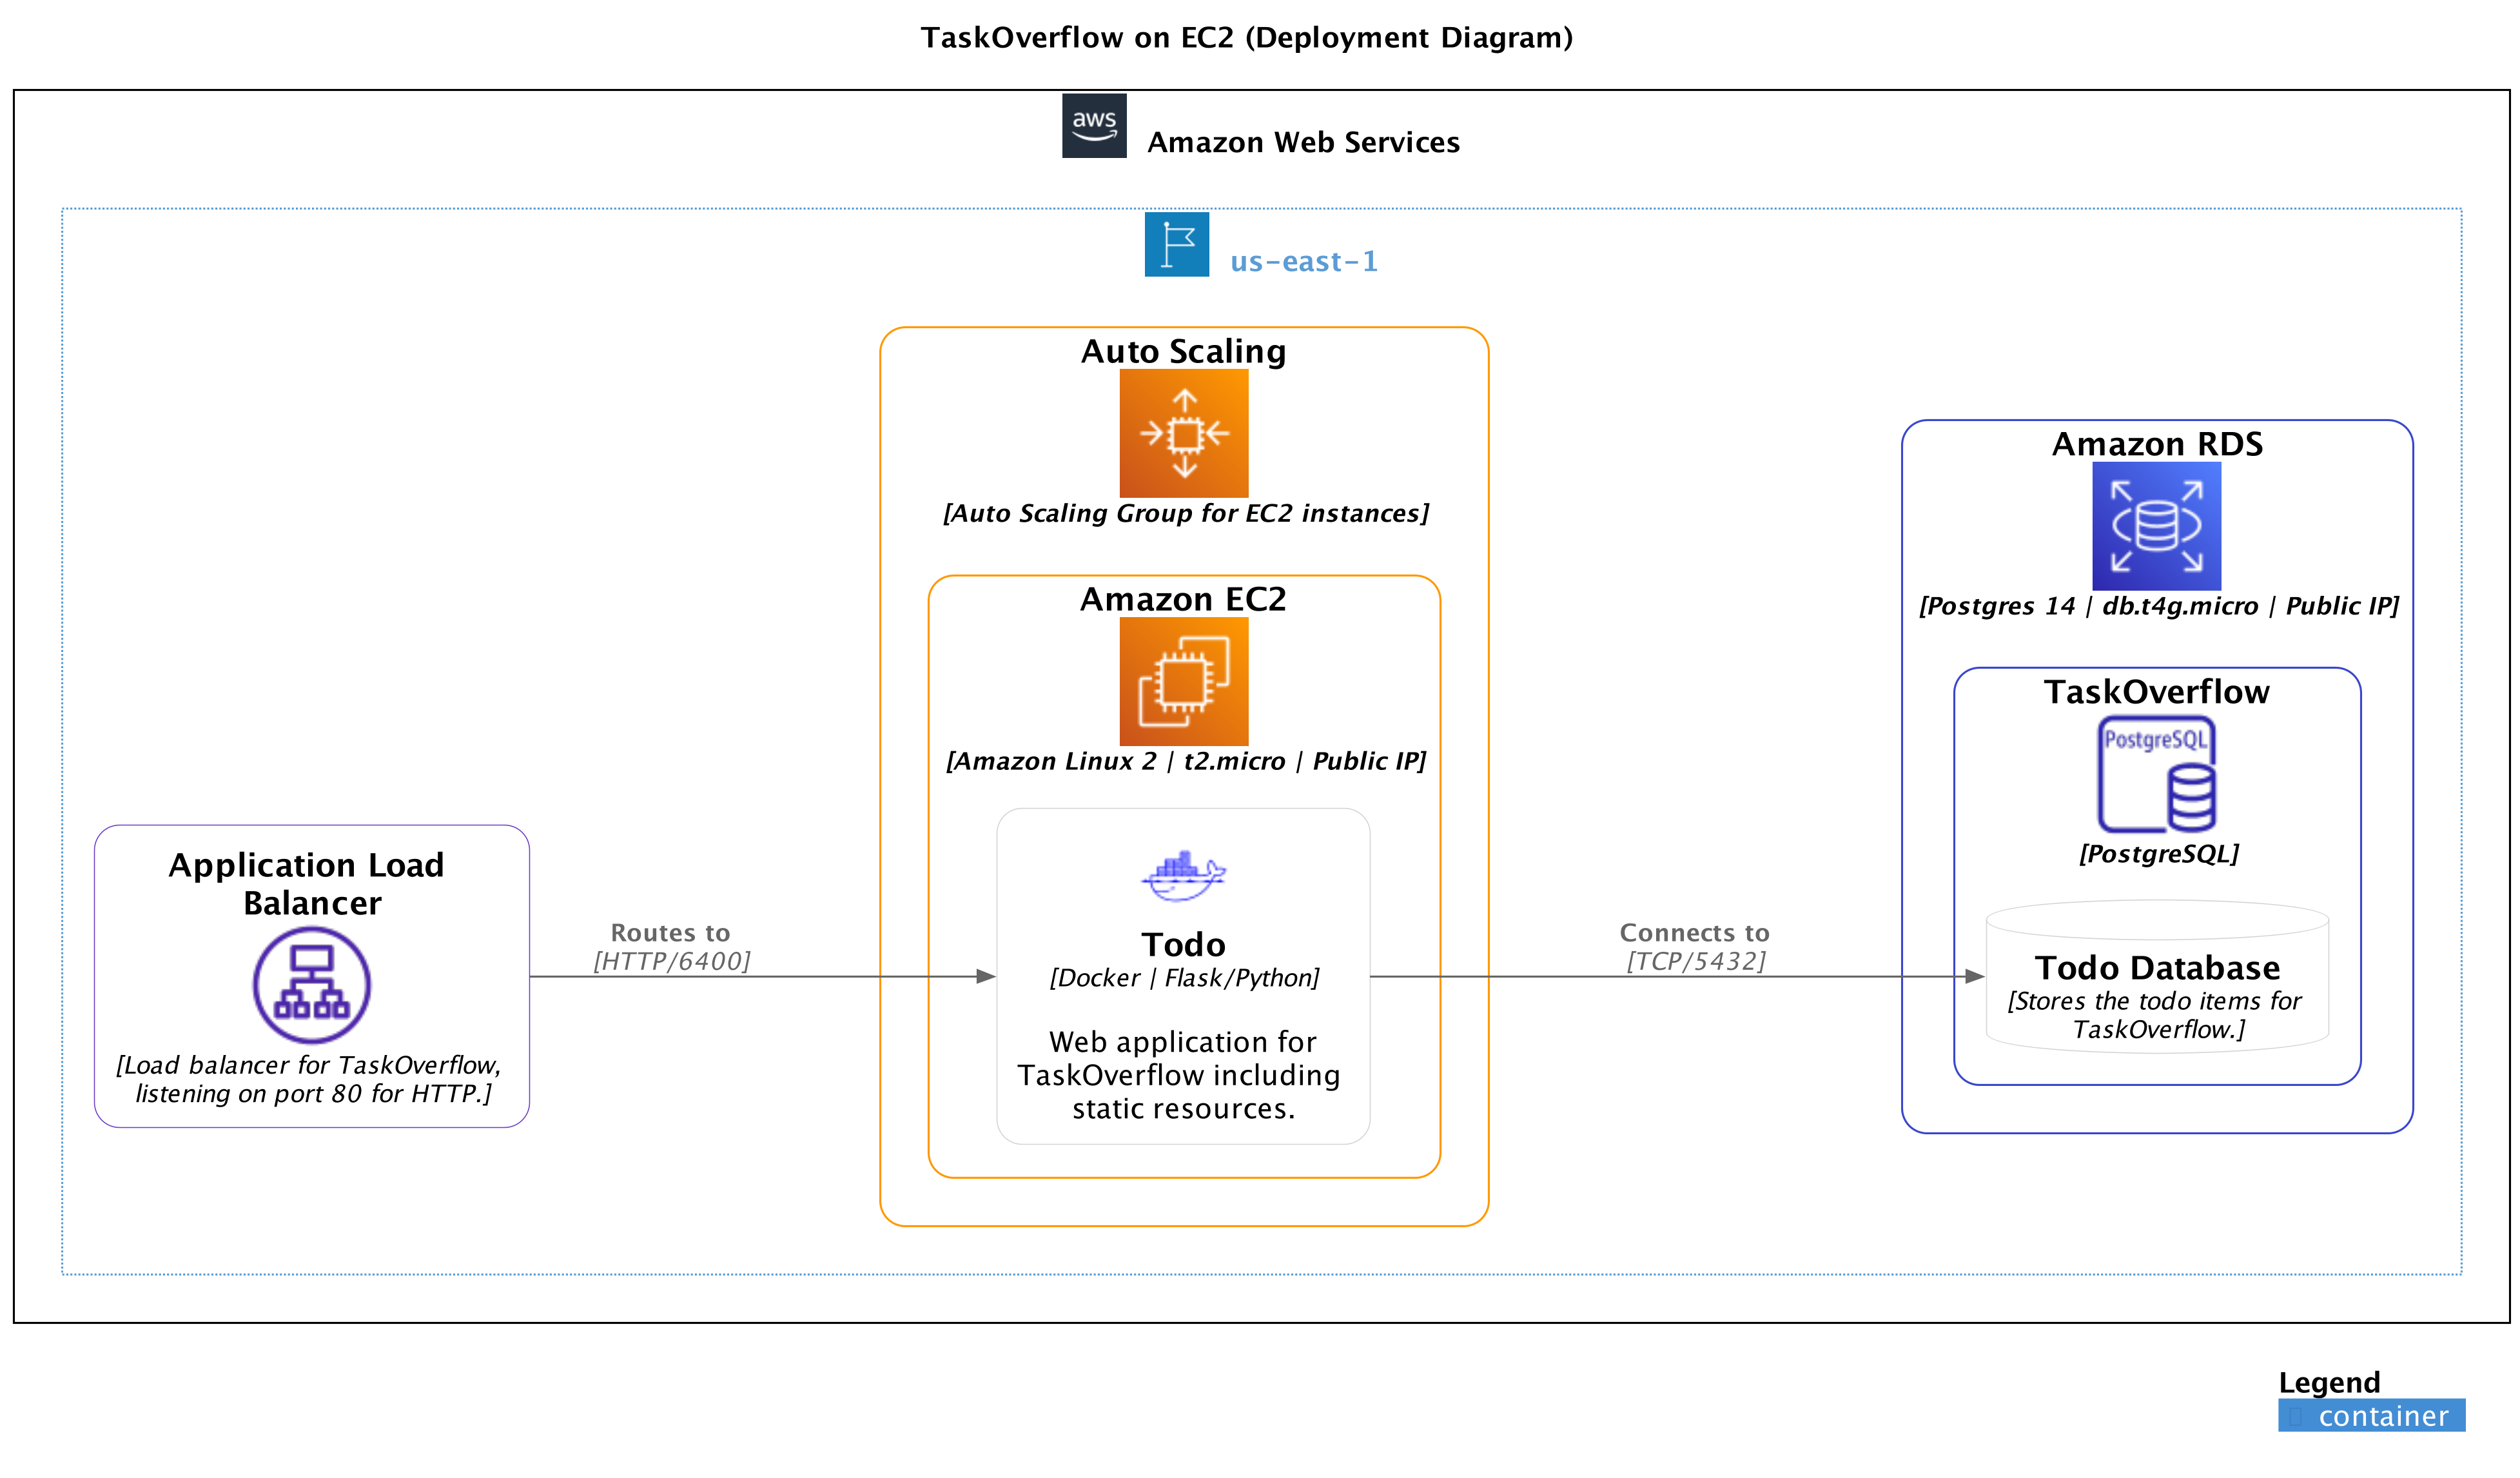
\includegraphics[width=\textwidth]{diagrams/ec2deployment}
\end{figure}

\todo{Move to EC2Template}

\todo{AutoScaling group}

\todo{target group}

\todo{autoscaling + target}

\todo{load balancer}

\todo{listener}

\todo{Applying autoscaling rules}

\subsection{[Path B] ECS}

\todo{load balancer}

\todo{adding to ecs}

\todo{listener}

\todo{Applying autoscaling rules}

\begin{figure}[H]
  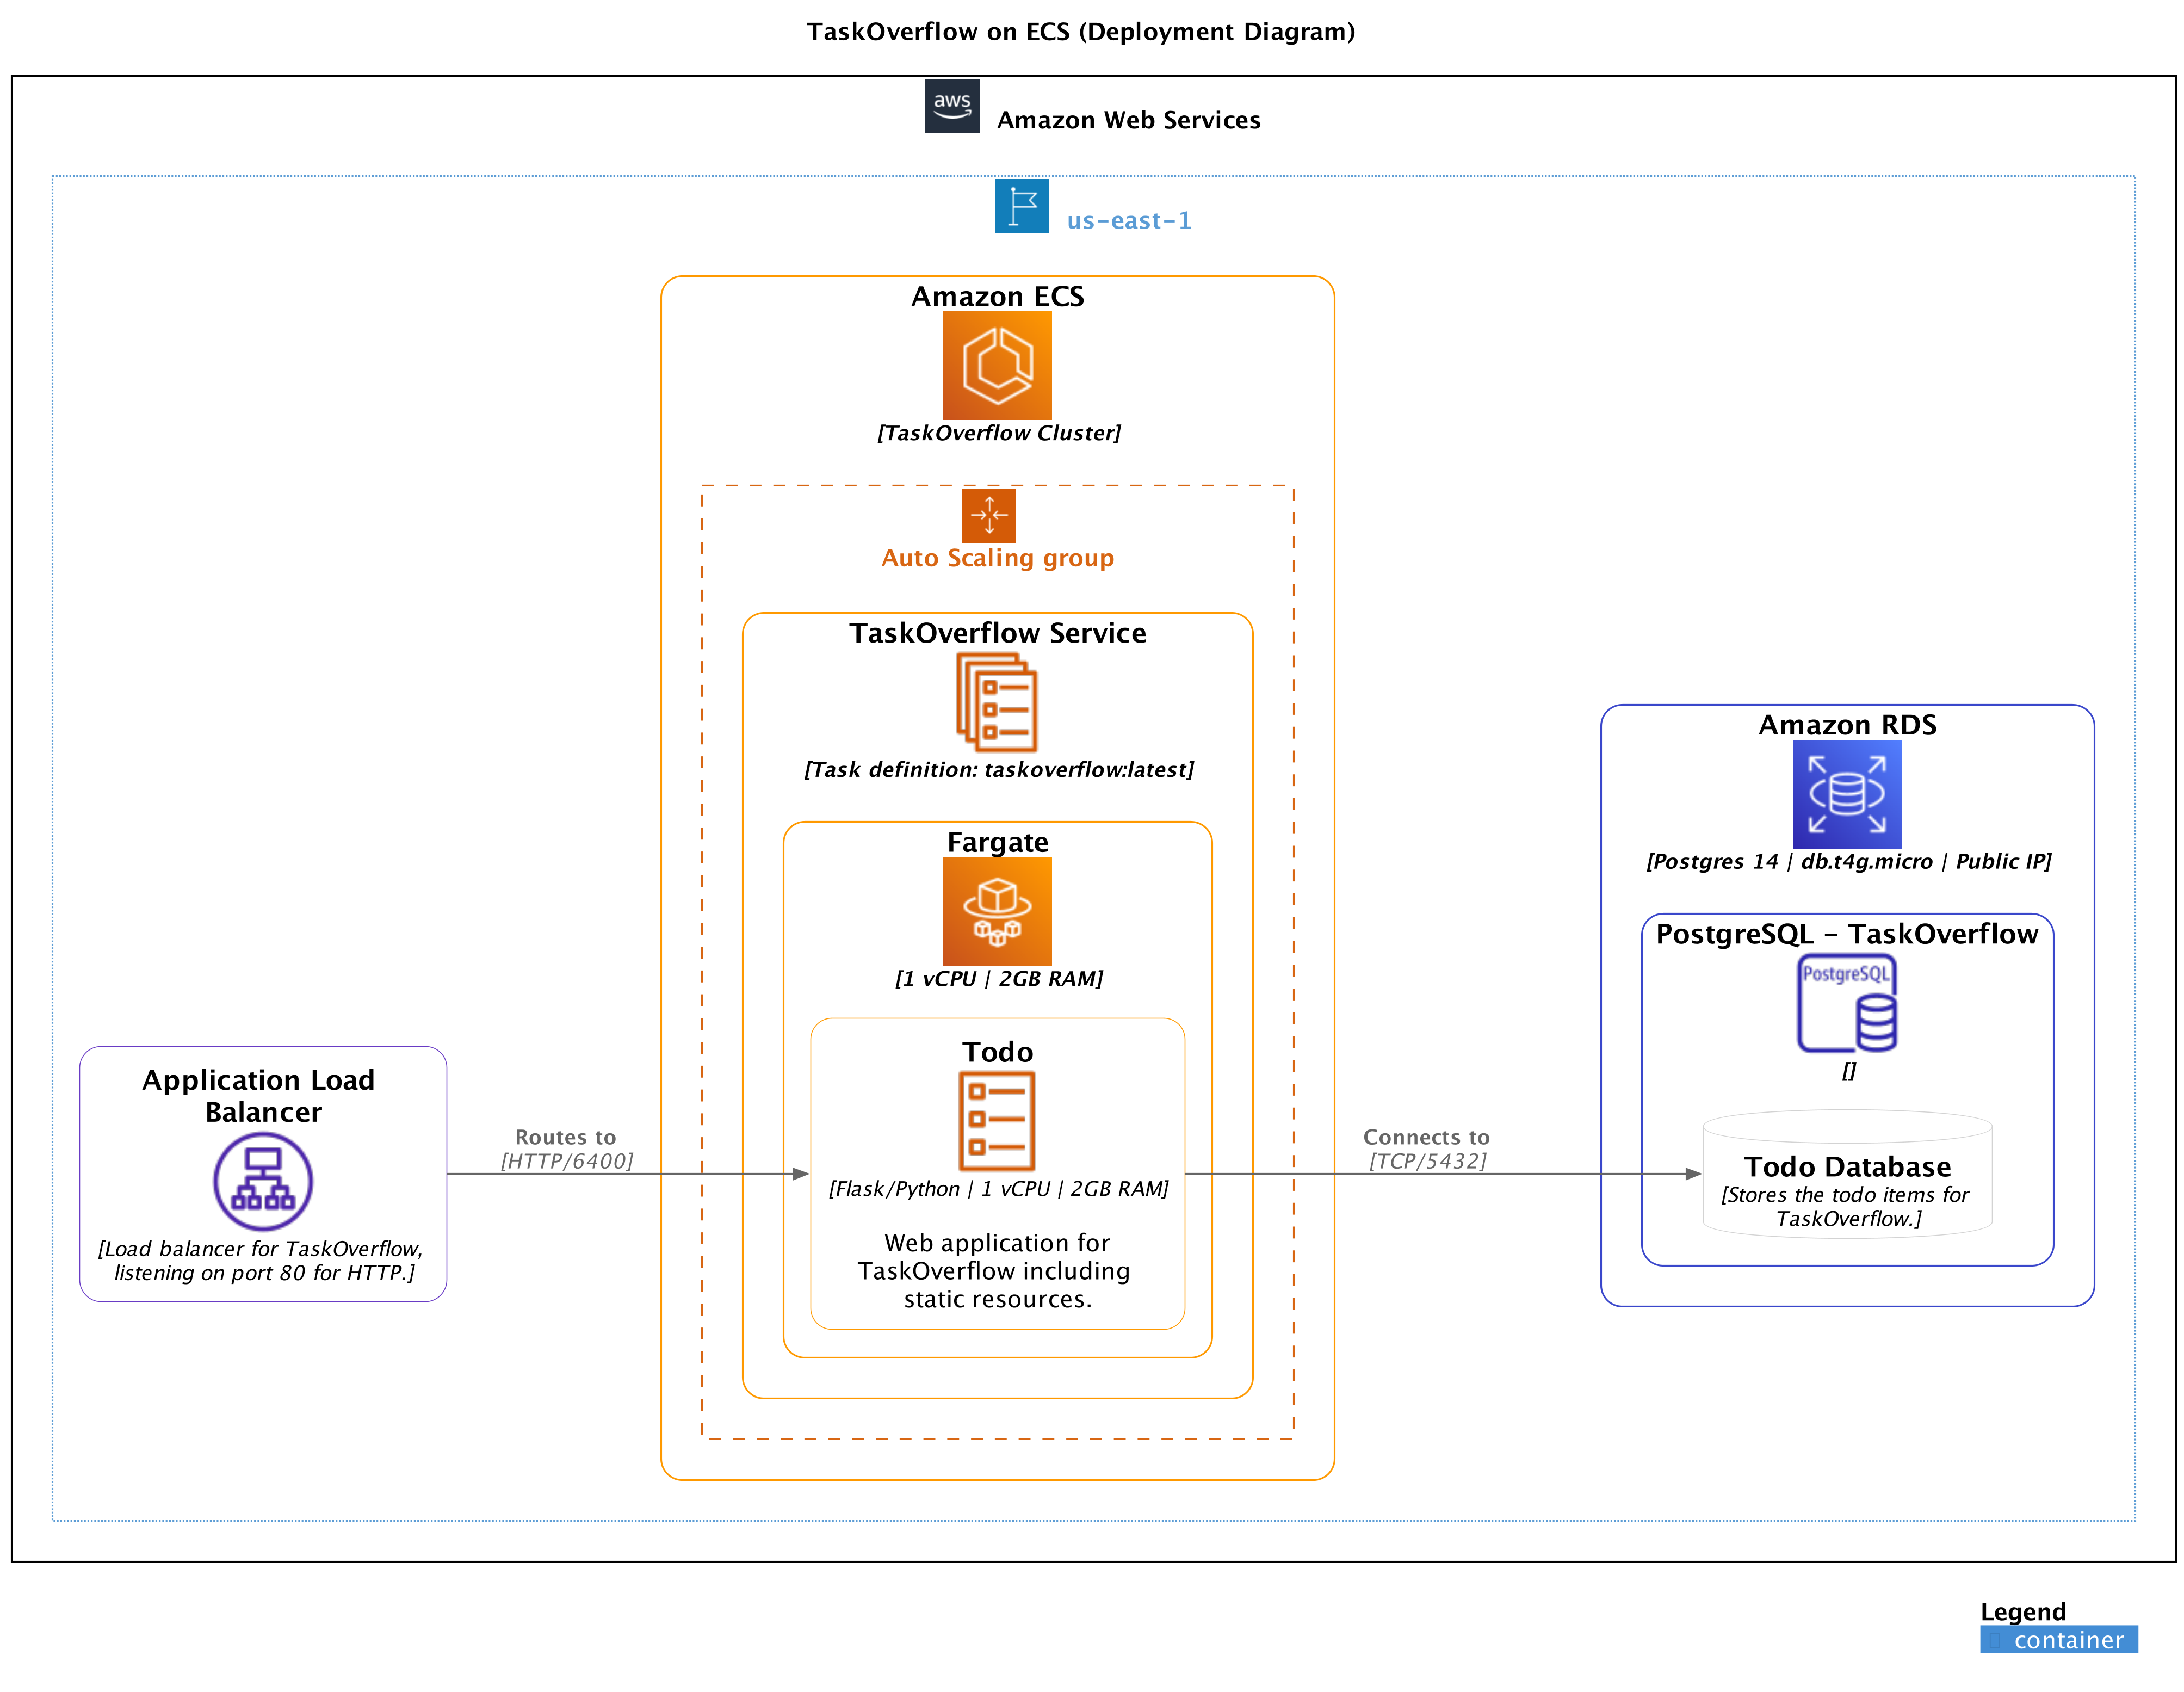
\includegraphics[width=\textwidth]{diagrams/ecsdeployment}
\end{figure}

\subsection{Producing Load with K6}


\bibliographystyle{ieeetr}
\bibliography{books,ours}

\end{document}